\documentclass{article}
\topmargin 0pt
\advance \topmargin by -\headheight
\advance \topmargin by -\headsep
\textheight 8.9in
\usepackage{color}
\usepackage{amsmath}
\usepackage{amsfonts}
\usepackage[noae]{Sweave}
\usepackage{enumerate}
\oddsidemargin 0pt
\evensidemargin \oddsidemargin

\begin{document}
\title{ CSCI-B 565 DATA MINING \\
Homework 3 \\
Morning Class\\
Computer Science Core\\Fall 2013\\Indiana University}
\author{ Debpriya Seal\\ debseal@indiana.edu}
\maketitle
All the work herein is solely mine. \\

\section*{Problem One}
		Assume you have a data series $ \Delta= a, b, a, b, b, a,? , a, b, b$ where the ? is missing data. Explain how to
replace this using uniform distribution, random distribution imputed from the data, and $B(p,n)$ .What are the sigificant differences between these three approaches? \\
	\emph{Answer:} 
	\begin{enumerate}
		\item Uniform Distribution.\\
		\emph{Answer:} Since we are given that the above distribution is unifrom. Then that means the chances of each is random variable is equal. Now, in the given distribution we have $P(a) = 4/9$ and $P(b) = 5/9$. So for the uniform distribution to hold the missing number should be a.

		\item Random Distribution.\\
		\emph{Answer:} Since we are given that the above distribution is random. However, looking at the data, clearly b appeared more number of times than a. So we can keeping that in mind we can say that the missing number is b.

		\item Bernoulli Distribution.\\
		\emph{Answer:} Since we are given that the above distribution is Bernoulli. Clearly, the data gives us the probability of 
getting a is $P(a) = 4/9 \text{ and } \\P(b) = 5/9$. Hence, clearly based on the probability we can easily say that the missing value is b.
	\end{enumerate}	


\section*{Problem Two: Medical Data}
\begin{enumerate}
	\item Write a reasonably formal statement that uses $\Delta$. What is the size of $\Delta$?\\
	\emph{Answer:} The size of delta is 699 tuples. Below is the formal statement: 
	This is data is about the breast cancer. And looking at the data we few things pop up straight away. Firstly that the data has been binned. As all the feautres apart from SCN are between 1 to 10. This rarely happens in real life. Also, the data look pretty clean.The task in our hand is to cluster these data into malignant or benign. The size of data is not huge by any standard. Also, the number of attributes we have is 10, however, not considering SCN we have 9 attributes. Compared to the size, these many attributes is a great thing.  For clustering I intend to use k-means algorithm as it one of most popular algorithm.Reason being is realitvely efficient with the running time complexity of $O(irck)$ where k is the number of clusters, i is the number of iterations, c is the number of features and r is the number of datapoints. 
	\begin{enumerate}
		\item Is this a large data set?\\
		\emph{Answer:} Well what is large is relative. What is large to me maynot be large to someone else. However, with huge RAM coming by. The defination of large has changed over time. Like the 3rd question given to us would be an example of large dataset. Since we have approximatly a million datapoints and 7K centroids. But I will go forward and say that it is not a large dataset by any means.\\
		\item Discuss the number of attributes with the data’s size\\
		\emph{Answer:} For this problen statement the number of attributes is 9 and number of datapoints is 699. Looking deeper inot k-means algorithm( which we are going to implement). The heart of k-means has a $C \times \Delta$ operation, where C is the number of centroids(which again is 2). So if we see the total operation approximatly is $2\times 699 = 1398$. And this in current computer speed is nothing. However, features does effect the result of the clustering algorithm. And you can see this clearly in the $5^th$question. If the number of features decreasing the accuracy will also start to decrease. \\
Lastly, For our astronomy data it would be $700 \times 0.7 \text{ million}= 70 \text{ million}$. Now that's huge by any standards.

	\end{enumerate}
	\item Ignoring the Sample code number (SCN), how many attributes does $\Delta$ have?\\
	\emph{Answer:} Ignoring the SCN, there are 9 attributes. The last one Class is not an attribute as it is the Label $y$.

	\item How many missing values are there? Give the SCNs for that have missing data. Remove the tuples that have missing data. Let $\Delta^{*}$  be a cleaned $\Delta$: the tuples with the missing values are removed. R offers several ways to remove unknown data, though you are free to write your own code. Let $\Delta^{m}= \Delta - \Delta^{*}$. For each $d \in \Delta^{m}$, replace the unknown data using one of the techniques we discussed in class; alternatively, you may employ your won approach. No matter how you decide to replace the unknowns, explain fully. The final data should be presented as $(SCN,A_{i}, data)$ where SCN is the tuple key, $A_i$ is the attribute, and data is the new data.\\


	\emph{Answer:} There are 16 missing values and all for $6^{th}$  attribute.Below is the output from my Java code.\\
\texttt{
Cleansing data .....\\
==============================================================
\begin{enumerate}[1.]
\item For SCN 1057013 attribute 6 for record 24 cleaned with 3
\item For SCN 1096800 attribute 6 for record 41 cleaned with 3
\item For SCN 1183246 attribute 6 for record 140 cleaned with 3
\item For SCN 1184840 attribute 6 for record 146 cleaned with 3
\item For SCN 1193683 attribute 6 for record 159 cleaned with 3
\item For SCN 1197510 attribute 6 for record 165 cleaned with 3
\item For SCN 1241232 attribute 6 for record 236 cleaned with 3
\item For SCN 169356 attribute 6 for record 250 cleaned with 3
\item For SCN 432809 attribute 6 for record 276 cleaned with 3
\item For SCN 563649 attribute 6 for record 293 cleaned with 3
\item For SCN 606140 attribute 6 for record 295 cleaned with 3
\item For SCN 61634 attribute 6 for record 298 cleaned with 3
\item For SCN 704168 attribute 6 for record 316 cleaned with 3
\item For SCN 733639 attribute 6 for record 322 cleaned with 3
\item For SCN 1238464 attribute 6 for record 412 cleaned with 3
\item For SCN 1057067 attribute 6 for record 618 cleaned with 3
\end{enumerate}
==============================================================\\
}\\
\textbf{Explanation over replacing data:} I decided to use mean of the attributes for which we have missing values. And it is a lot better than getting rid of missing data. Particularly, with small data, getting rid of data has substantial effect. 

\textbf{R code for getting rid of data with missing values:}
\begin{Sinput}
>myData <- read.table("WolBergsBreastCancerData.csv", sep=",", 
+ header = FALSE, colClasses=c("character", "character",
+ "character","character","character","character", +"character", 
+ "character", "character", "character", "character"), 
+ na.strings=c("NA","?"))
>cleanData <- na.omit(myData)
\end{Sinput}
	\begin{enumerate}
		\item Is the amount of missing data significant? \\
		\emph{Answer:} The total amount of datapoints we have is 699. ANd among them 16 are missing. So it comes about $2.3\%$, and missing value within 1-5\% is considered to be managebale.  Although significant is a relative word. And its defination differ person to person. However, for me it is not that significant. 
		\item Assess the significance of either keeping or removing the tuples with unknown data.\\
		\emph{Answer:} It is always good to keep the data by replacing with some other values rather than just getting rid of it. And it becomes more significant if the amount of missing data is huge. Then getting rid of them is not a prudent choice.Moreover, even though an attribute is missing in a datapoint but other attributes are still present.With insufficient data, removal might lead to biased results.\\
On the other hand, imputing the mean/median for missing values is generally common practice. Although, it is better than just throwing away the data. But it has its own problems. By replacing the missing values with a mean/median we distort the actual distribution.And this happen to work for me. \\
\\Below you can see how much adverse effect throwing the data out has on small dataset.

		\begin{table}[h]
			\caption{PPV by Number of attribute with \textbf{Mean} Imputation}

			\centering
			\begin{tabular}{c|c c}
				\\
				\hline
				$C_{km=2} (\Delta^*)$ & \# of Iteration to Converge & PPV \\
				\hline
				$A_1, . . . , A_9$ & 3 & 0.9570815450643777\\
				$A_1, . . . , A_7$ & 3 & 0.9570815450643777\\
				$A_1, . . . , A_5$ & 6 & 0.9356223175965666\\
				$A_1, . . . , A_3$ & 5 & 0.932761087267525\\
				$A_1, A_2$  & 3 & 0.8869814020028612\\
				\hline	
			\end{tabular} \\
			*The missing value was replaced with 3
		\end{table}[h] \\			
		
		\begin{table}[h]
			\caption{PPV by Number of attribute with \textbf{Removal} of records with missing values}
			\centering
			\begin{tabular}{c|c c}
				\\
				\hline
				$C_{km=2} (\Delta^*)$ & \# of Iteration to Converge & PPV \\
				\hline
				$A_1, . . . , A_9$ & 4 & \textcolor{red}{0.7130307467057101}\\
				$A_1, . . . , A_7$ & 4 & \textcolor{red}{0.677891654465593}\\
				$A_1, . . . , A_5$ & 6 & \textcolor{red}{0.7569546120058566}\\
				$A_1, . . . , A_3$ & 4 & \textcolor{red}{0.7818448023426061}\\
				$A_1, A_2$  & 4 & \textcolor{red}{0.7569546120058566}\\
				\hline	
			\end{tabular}\\
			*The missing value records were thrown away
		\end{table}[h] \\	
		\pagebreak
	\end{enumerate}

	\item Assume the attribute Clump Thickness is $A_1$, Uniformity of Cell Size is $A_2$ and so on. Attribute $A_10$ has only two domain values and is the classifier. For $\Delta^*$ and the attributes $A_i , 1 \le i \le 9$.
	\begin{enumerate}
		\item Which $A_i$ has the greatest variance? You will write an R function that takes a list of numbers and returns the variance. \\
		\emph{Answer:} I wrote a R function which takes variance or entropy as argument and returns the attribute.\\

By removing the tuples with missing values:
\begin{Sinput}
> operFuncOnAttr("WolBergsBreastCancerData.csv", "var","y")
\end{Sinput}
\begin{Soutput}
V7 
 6 
\end{Soutput}

By replacing attributes with missing values with Mean:
\begin{Sinput}
> operFuncOnAttr("WolBergsBreastCancerData.csv", "var","n")
\end{Sinput}
\begin{Soutput}
V7 
 6 
\end{Soutput}

		\item Which $A_i$ has the lowest entropy? You may use the R package entropy by Hausser and Strimmer. \\
		\emph{Answer:} 
By removing the tuples with missing values:\\
\begin{Sinput}
> operFuncOnAttr("WolBergsBreastCancerData.csv", "entropy","n")
\end{Sinput}
\begin{Soutput}
V9 
 8  
\end{Soutput}

By replacing attributes with missing values with Mean:\\
\begin{Sinput}
> operFuncOnAttr("WolBergsBreastCancerData.csv", "entropy","y")
\end{Sinput}
\begin{Soutput}
V9 
6
\end{Soutput}

\textbf{R code for function operFuncOnAttr:}
\begin{Sinput}

operFuncOnAttr <- function (fileName, funct, removeAttr) {

	#Reading the file and storing it in a Dataset
	myData <- read.table(fileName, sep=",", header = FALSE, 
+ colClasses=c("character","character","character","character","character",
+ "character","character","character","character","character","character"), 
+ na.strings=c("NA","?"))
	
	#Ignoring the SCN for the computation
	myData <- myData[, 2:(ncol(myData)-1)]
	
	# Converting string to numeric.
	cols <- c(1:(ncol(myData)))
	myData[,cols] = apply(myData[,cols], 2, function(x) as.numeric(x))
	
	#replacing the tuples with missing values with mean.
	if (removeAttr == "n"){
	myData[is.na(myData)] <- mean(myData[,6], na.rm=TRUE)
	}
	
	if (funct == "var") {
		ret <- which.max(sapply (myData, var,na.rm=TRUE))
	} else {
		# load entropy library
		if(is.element("entropy", installed.packages()[,1])) { 
			print("entropy package already installed") 
		} else {
			print("Installing Package entropy ....") 
			install.packages('entropy')
		}
		library("entropy")
		ret <- which.min(sapply(myData, entropy,na.rm=TRUE))
	}
	return (ret)
}
\end{Sinput}


		\item Fill-in the table below with the KL distance for attribute pairs. For this we construct a mass function $P_i$ over $A_i$ by simple counting. For a cell whose row, column entries are $A_i,A_j$, find $d_{KL}(P_i||P_j)$. You may use an existing R function for this, but you need to provide sufficient package details for someone who would consider using that package.\\
		\emph{Answer:}
		\begin{enumerate}	
			\item When throwing away the tuples the KL Distance Matrix looks like:
\begin{Sinput}
> computeKLDist("WolBergsBreastCancerData.csv","y")
\end{Sinput}			
\begin{Soutput}			
[1] "seewave package already installed"
           [,1]       [,2]       [,3]      [,4]      [,5]      [,6]      [,7]
 [1,] 0.0000000 0.34942479 0.32526209 0.4602240 0.2598199 0.4825389 0.2953075
 [2,] 0.3303850 0.00000000 0.09345295 0.3017260 0.2293274 0.3406523 0.2406133
 [3,] 0.3131351 0.09296301 0.00000000 0.3226041 0.2367744 0.3262189 0.2470536
 [4,] 0.4488371 0.27668360 0.29780869 0.0000000 0.3332852 0.3821307 0.3154832
 [5,] 0.2791672 0.23689648 0.24479753 0.3526845 0.0000000 0.4329557 0.2250175
 [6,] 0.4430740 0.30147808 0.28623300 0.3850621 0.4006527 0.0000000 0.3421348
 [7,] 0.3017020 0.24714584 0.25332848 0.3138671 0.2118222 0.3761513 0.0000000
 [8,] 0.4493107 0.27416155 0.27801764 0.4282573 0.3354324 0.4702960 0.3271679
 [9,] 0.4898512 0.48282164 0.50148291 0.5492319 0.3456823 0.6821753 0.4828394
\end{Soutput}

\begin{Soutput}
          [,8]      [,9]
 [1,] 0.4827846 0.4339470
 [2,] 0.3246805 0.5338144
 [3,] 0.3324193 0.5311455
 [4,] 0.4421757 0.5593252
 [5,] 0.3628460 0.3457609
 [6,] 0.5023946 0.6797457
 [7,] 0.3645522 0.4533546
 [8,] 0.0000000 0.5868865
 [9,] 0.5418213 0.0000000
\end{Soutput}
	\item When repalcing the missing values with mean the KL Distance Matrix looks like:
\begin{Sinput}
> computeKLDist("WolBergsBreastCancerData.csv","n")
\end{Sinput}			
\begin{Soutput}			
[1] "seewave package already installed"
           [,1]       [,2]       [,3]      [,4]      [,5]      [,6]      [,7]
 [1,] 0.0000000 0.34738153 0.32400762 0.4641627 0.2617773 0.4812723 0.2923631
 [2,] 0.3281002 0.00000000 0.09438032 0.3058258 0.2316805 0.3450263 0.2407317
 [3,] 0.3113454 0.09473766 0.00000000 0.3283380 0.2382599 0.3272561 0.2454988
 [4,] 0.4516002 0.27842612 0.30137452 0.0000000 0.3310688 0.3886677 0.3182790
 [5,] 0.2808857 0.23827180 0.24550698 0.3496033 0.0000000 0.4308768 0.2258272
 [6,] 0.4433625 0.30757052 0.28902232 0.3904466 0.3977981 0.0000000 0.3398343
 [7,] 0.2980436 0.24713276 0.25208530 0.3180932 0.2128848 0.3733125 0.0000000
 [8,] 0.4476825 0.26963252 0.27628375 0.4311402 0.3374148 0.4754893 0.3271676
 [9,] 0.4890809 0.48393551 0.50151244 0.5485056 0.3443245 0.6750230 0.4808986

           [,8]      [,9]
 [1,] 0.4815181 0.4329595
 [2,] 0.3202202 0.5343926
 [3,] 0.3305491 0.5294709
 [4,] 0.4421630 0.5608295
 [5,] 0.3633375 0.3445298
 [6,] 0.5062158 0.6672949
 [7,] 0.3639762 0.4505998
 [8,] 0.0000000 0.5919925
 [9,] 0.5458185 0.0000000\end{Soutput}
		\end{enumerate}	
	\end{enumerate}

	\item Implement k-means (see Algorithm1) so that you can cluster $\Delta^*$. Call this program $C_km$. For this first iteration, you may assume that $1 \le k \le 10$ and that all domain values are numeric. Write $C_{km=i}$ for i blocks (or clusters). Assume there are k blocks $C_1, C_2, . . . , C_k$. If an element of $C_i$ is correctly clustered in $C_i$, then it is considered a True Positive (TP). If an element that correctly belongs to $C_i$ is clustered in a different $C_j$ , then the element is a False Positive (FP). The Positive Predictive Value (PPV) is \\
$ PPV = \frac{TP}{TP+FP}$
In this problem we will investigate $C_{km’s}$ PPV varying the attributes used. Specifically, create a table that pairs $C_{km=2’s}$ PPV using the attributes shown in the table below:\\
	\emph{Answer:} 
Since the first part of the questions says that the $1\le k \le 10$. I ran k-means with 9 attributes for cluster 1 to n. And below are the accuracies. 
			\begin{table}[h]
				\caption{K-means for clusters from 1 to 10}

				\centering
				\begin{tabular}{c|cc}
					\\
					\hline
					$C_{km=i} (\Delta^*)$ & \# of Iteration to Converge & PPV \\
					\hline
					$C_{km=1}$ & 1 & 0.6552217453505007\\
					$C_{km=2}$ & 5 & 0.9570815450643777\\
					$C_{km=3}$ & 10 & 0.9628040057224606\\
					$C_{km=4}$ & 14 & 0.9570815450643777\\
					$C_{km=5}$  & 9 & 0.9699570815450643\\
					$C_{km=6}$  & 16 & 0.9599427753934192\\
					$C_{km=7}$  & 11 & 0.9699570815450643\\
					$C_{km=8}$  & 9 & 0.9713876967095851\\
					$C_{km=9}$  & 14 & 0.9699570815450643\\
					$C_{km=10}$  & 12 & 0.9656652360515021\\
					\hline	
				\end{tabular} \\
				*The missing value was replaced with 3
			\end{table}[h] \\	
			\textbf{Analysis:} I was amazed to see the k-means to cluster every single time. Even though the PPV will not make sense here. But the fact that it converged every single time is amazing. 		



			\begin{table}[h]
				\caption{PPV by Number of attribute with \textbf{Mean} Imputation}

				\centering
				\begin{tabular}{c|c c}
					\\
					\hline
					$C_{km=2} (\Delta^*)$ & \# of Iteration to Converge & PPV \\
					\hline
					$A_1, . . . , A_9$ & 3 & 0.9570815450643777\\
					$A_1, . . . , A_7$ & 3 & 0.9570815450643777\\
					$A_1, . . . , A_5$ & 6 & 0.9356223175965666\\
					$A_1, . . . , A_3$ & 5 & 0.932761087267525\\
					$A_1, A_2$  & 3 & 0.8869814020028612\\
					\hline	
				\end{tabular} \\
				*The missing value was replaced with 3
			\end{table}[h] \\			

			\begin{table}[h]
				\caption{PPV by Number of attribute with \textbf{Median} Imputation}
				\centering
				\begin{tabular}{c|c c}
					\\
					\hline
					$C_{km=2} (\Delta^*)$ & \# of Iteration to Converge & PPV \\
					\hline
					$A_1, . . . , A_9$ & 6 & \textcolor{red}{0.9585121602288984}\\
					$A_1, . . . , A_7$ & 4 & 0.9570815450643777\\
					$A_1, . . . , A_5$ & 5 & 0.9356223175965666\\
					$A_1, . . . , A_3$ & 3 & 0.932761087267525\\
					$A_1, A_2$  & 7 & 0.8869814020028612\\
					\hline	
				\end{tabular}\\
				*The missing value was replaced with 1
			\end{table}[h] \\	


			\begin{table}[h]
				\caption{PPV by Number of attribute with \textbf{Mode} Imputation}
				\centering
				\begin{tabular}{c|c c}
					\\
					\hline
					$C_{km=2} (\Delta^*)$ & \# of Iteration to Converge & PPV \\
					\hline
					$A_1, . . . , A_9$ & 6 & \textcolor{red}{0.9585121602288984}\\
					$A_1, . . . , A_7$ & 3 & 0.9570815450643777\\
					$A_1, . . . , A_5$ & 5 & 0.9356223175965666\\
					$A_1, . . . , A_3$ & 3 & 0.932761087267525\\
					$A_1, A_2$  & 4 & \textcolor{red}{0.8841201716738197}\\
					\hline	
				\end{tabular}\\
				*The missing value was replaced with 1
			\end{table}[h] \\	


			\begin{table}[h]
				\caption{PPV by Number of attribute with \textbf{Removal} of records with missing values}
				\centering
				\begin{tabular}{c|c c}
					\\
					\hline
					$C_{km=2} (\Delta^*)$ & \# of Iteration to Converge & PPV \\
					\hline
					$A_1, . . . , A_9$ & 4 & \textcolor{red}{0.7130307467057101}\\
					$A_1, . . . , A_7$ & 4 & \textcolor{red}{0.677891654465593}\\
					$A_1, . . . , A_5$ & 6 & \textcolor{red}{0.7569546120058566}\\
					$A_1, . . . , A_3$ & 4 & \textcolor{red}{0.7818448023426061}\\
					$A_1, A_2$  & 4 & \textcolor{red}{0.7569546120058566}\\
					\hline	
				\end{tabular}\\
				*The missing value records were thrown away
			\end{table}[h] \\	
	\pagebreak
	\item One of the most common techniques in assessing function is using V -fold cross validation. The idea is simple. Suppose $\Delta^*$ = N. Partition $\Delta^*$  into V = 10 sets $D^*= {d_1^*, d_2^* , . . . , d_10^*}$ such that each $|d_i^* | = N/10$ tuples and all $d_i, d_j$ are pairwise disjoint. The task is to use V − 1 sets to  train and the remaining d to test. Fill-in the PPV for each fold. Create a weighted PPV, $(1/10)\sum_ {i=1}^{10}PPV_ i$\\
	\emph{Answer:} 
			\begin{table}[h]
				\caption{PPV over V-fold with \textbf{Mean} Imputation}

				\centering
				\begin{tabular}{c||c| c|c}
					\\
					\hline
					Train & \# of Iteration to Converge & Test & PPV Results\\
					\hline
					$C_{km=2}(D^* - d^*_1)$ & 5 & $C_{km=2}( d^*_1)$&0.8142857142857143\\
					$C_{km=2}(D^* - d^*_2)$ & 5 & $C_{km=2}( d^*_2)$&0.9571428571428572\\
					$C_{km=2}(D^* - d^*_3)$ & 6 & $C_{km=2}( d^*_3)$&0.9857142857142858\\
					$C_{km=2}(D^* - d^*_4)$ & 7 & $C_{km=2}( d^*_4)$&0.9428571428571428\\
					$C_{km=2}(D^* - d^*_5)$ & 4 & $C_{km=2}( d^*_5)$&0.9428571428571428\\
					$C_{km=2}(D^* - d^*_6)$ & 5 & $C_{km=2}( d^*_6)$&0.9714285714285714\\
					$C_{km=2}(D^* - d^*_7)$ & 5 & $C_{km=2}( d^*_7)$&0.9571428571428572\\
					$C_{km=2}(D^* - d^*_8)$ & 5 & $C_{km=2}( d^*_8)$&1.0\\
					$C_{km=2}(D^* - d^*_9)$ & 6 & $C_{km=2}( d^*_9)$ &1.0\\
					$C_{km=2}(D^* - d^*_10)$ & 4 & $C_{km=2}( d^*_10)$&1.0\\
					\hline	
				\end{tabular} \\
				*Weighted PPV = 0.9571428571428573
			\end{table}[h] \\			

			\begin{table}[h]
				\caption{PPV over V-fold with \textbf{Median} Imputation}

				\centering
				\begin{tabular}{c||c| c|c}
					\\
					\hline
					Train & \# of Iteration to Converge & Test & PPV Results\\
					\hline
					$C_{km=2}(D^* - d^*_1)$ & 6 & $C_{km=2}( d^*_1)$&0.8142857142857143\\
					$C_{km=2}(D^* - d^*_2)$ & 4 & $C_{km=2}( d^*_2)$&0.9571428571428572\\
					$C_{km=2}(D^* - d^*_3)$ & 4 & $C_{km=2}( d^*_3)$&0.9857142857142858\\
					$C_{km=2}(D^* - d^*_4)$ & 8 & $C_{km=2}( d^*_4)$&0.9428571428571428\\
					$C_{km=2}(D^* - d^*_5)$ & 5 & $C_{km=2}( d^*_5)$&0.9428571428571428\\
					$C_{km=2}(D^* - d^*_6)$ & 5 & $C_{km=2}( d^*_6)$&0.9714285714285714\\
					$C_{km=2}(D^* - d^*_7)$ & 4 & $C_{km=2}( d^*_7)$&0.9571428571428572\\
					$C_{km=2}(D^* - d^*_8)$ & 4 & $C_{km=2}( d^*_8)$&1.0\\
					$C_{km=2}(D^* - d^*_9)$ & 3 & $C_{km=2}( d^*_9)$ &1.0\\
					$C_{km=2}(D^* - d^*_10)$ & 5 & $C_{km=2}( d^*_10)$&1.0\\
					\hline	
				\end{tabular} \\
				*Weighted PPV = 0.9571428571428573
			\end{table}[h] \\			

			\begin{table}[h]
				\caption{PPV over V-fold with \textbf{Mode} Imputation}

				\centering
				\begin{tabular}{c||c| c|c}
					\\
					\hline
					Train & \# of Iteration to Converge & Test & PPV Results\\
					\hline
					$C_{km=2}(D^* - d^*_1)$ & 5 & $C_{km=2}( d^*_1)$&0.8142857142857143\\
					$C_{km=2}(D^* - d^*_2)$ & 3 & $C_{km=2}( d^*_2)$&0.9571428571428572\\
					$C_{km=2}(D^* - d^*_3)$ & 4 & $C_{km=2}( d^*_3)$&0.9857142857142858\\
					$C_{km=2}(D^* - d^*_4)$ & 6 & $C_{km=2}( d^*_4)$&0.9428571428571428\\
					$C_{km=2}(D^* - d^*_5)$ & 5 & $C_{km=2}( d^*_5)$&0.9428571428571428\\
					$C_{km=2}(D^* - d^*_6)$ & 5 & $C_{km=2}( d^*_6)$&0.9714285714285714\\
					$C_{km=2}(D^* - d^*_7)$ & 5 & $C_{km=2}( d^*_7)$&0.9571428571428572\\
					$C_{km=2}(D^* - d^*_8)$ & 5 & $C_{km=2}( d^*_8)$&1.0\\
					$C_{km=2}(D^* - d^*_9)$ & 5 & $C_{km=2}( d^*_9)$ &1.0\\
					$C_{km=2}(D^* - d^*_10)$ & 5 & $C_{km=2}( d^*_10)$&1.0\\
					\hline	
				\end{tabular} \\
				*Weighted PPV = 0.9571428571428573
			\end{table}[h] \\		


			\begin{table}[h]
				\caption{PPV over V-fold with \textbf{Removal} of missing data tuple}

				\centering
				\begin{tabular}{c||c| c|c}
					\\
					\hline
					Train & \# of Iteration to Converge & Test & PPV Results\\
					\hline
					$C_{km=2}(D^* - d^*_1)$ & 3 & $C_{km=2}( d^*_1)$&0.5294117647058824\\
					$C_{km=2}(D^* - d^*_2)$ & 4 & $C_{km=2}( d^*_2)$&0.5882352941176471\\
					$C_{km=2}(D^* - d^*_3)$ & 5 & $C_{km=2}( d^*_3)$&0.6911764705882353\\
					$C_{km=2}(D^* - d^*_4)$ & 6 & $C_{km=2}( d^*_4)$&0.5294117647058824\\
					$C_{km=2}(D^* - d^*_5)$ & 5 & $C_{km=2}( d^*_5)$&0.5\\
					$C_{km=2}(D^* - d^*_6)$ & 5 & $C_{km=2}( d^*_6)$&0.8529411764705882\\
					$C_{km=2}(D^* - d^*_7)$ & 6 & $C_{km=2}( d^*_7)$&0.8088235294117647\\
					$C_{km=2}(D^* - d^*_8)$ & 6 & $C_{km=2}( d^*_8)$&0.8823529411764706\\
					$C_{km=2}(D^* - d^*_9)$ & 6 & $C_{km=2}( d^*_9)$ &0.7941176470588235\\
					$C_{km=2}(D^* - d^*_10)$ & 5 & $C_{km=2}( d^*_10)$&0.9705882352941176\\
					\hline	
				\end{tabular} \\
				*Weighted PPV = 0.7147058823529412
			\end{table}[h] \\		
\end{enumerate}
\pagebreak
\section*{Problem Three: Astronomy}

\begin{enumerate}[1.]
	\item Prove or disprove that R is a metric.\\
	\emph{Answer:}
		\item Lets  see whether the below distance is a metric or not\\
			$R(g,g^{'}) = \left((\frac{z_g - z_{g^{'}}}{0.2596})^2 + (\frac{r_g - r_{g^{'}}}{8.6})^2 + (\frac{(u_g - r_g) - (u_{g^{'}} - r_{g^{'}}) }{11.84})^2\right)^{1/2}$ \\
			In order to prove it is metric, we need to make sure that the above 4 properties are met. Let us see them one by one,\\
			\begin{enumerate}[(i)]
			\item $d(x, y) \ge 0$ for all $x, y \in X$: \\This is true since we are taking aquare of elements and adding them later on. Hence, it can never be less than 0.
			\item $d(x, y) = 0$ if and only if  $x = y$: \\Clearly since we are doing subtraction operation here. For it to be 0, $x=y$.
			\item $d(x, y) = d(y, x)$ for all $x, y \in X$: \\ Again taking square help us out here. Since, we are taking square, it really doesn't matter we take perform $x-y$ or $y-x$.
			\item $d(x, y) \ge d(x, z) + d(z, y)$ for all $x, y, z \in X$: \\ Lets observe our distance function more closely. Firstly, lets get rid of the constants.Since constants are not really going to be a problem to prove this.  Then we have the following equation. \\
			$R(g,g^{'}) = \left((z_g - z_{g^{'}})^2 + (r_g - r_{g^{'}})^2 + ((u_g - r_g) - (u_{g^{'}} -r_{g^{'}}))^2 \right)^{1/2}$ \\

Now. Lets call $(u_{g^{'}} -r_{g^{'}}) = a_{g^{'}}$, $(u_{g} -r_{g}) = a_{g}$; then we have :\\
			$R(g,g^{'}) = \left((z_g - z_{g^{'}})^2 + (r_g - r_{g^{'}})^2 + (a_g - a_{g^{'}})^2 \right)^{1/2}$ \\
Now what is this, this is nothing but eculidean distance in 3D space. And we know eculedian is a metric, so it should satisfy the transitivity rule.

Hence, proved that $R(g,g^{'})$ is a metric.

			\end{enumerate}

	\item Run the control algorithm and compare the output to control 2.\\
	\emph{Answer:} I ran the control algorithm and compared it with mine. Below is the output of the same from my Java Code:
	\begin{Soutput}
===============================================================
Computing control Algortihm......
Number of datapoints present in both    :0
Number of datapoints present only in our computed control       :7246
Number of datapoints present only in our given control  :7246
===============================================================
	\end{Soutput}

	\item Run k − means on candidate using main as the centroids. Because the galaxy type must be identical, you should first partition candidate into three blocks that represents galaxy types 0,1,2 and similarly for main. For each block in candidate, use the corresponding block in the partitioned main as the centroids.\\
	\emph{Answer:} Please see the .java file attached for this. Below is the few analysis i did before coding for the data.Although the plots did not came out to be really clear. Howver, it shows one important thing that we do have few outliers. Which stand apart in the 3d plot. \\
\textbf{NOTE:} I ahave not attached the candidate dataset plots. As they are upto 34MB in size and making latex to stop working. However, I plan to attach them along with other documents.
\begin{figure}
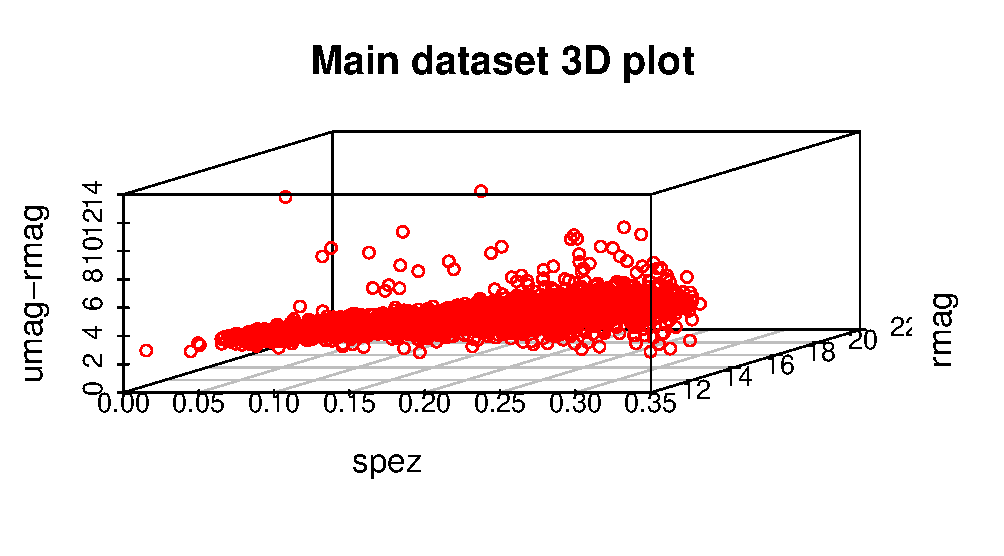
\includegraphics{main3dScatterPlot.pdf}
\caption{ 3D scatter plot for data in \emph{main} dataset}

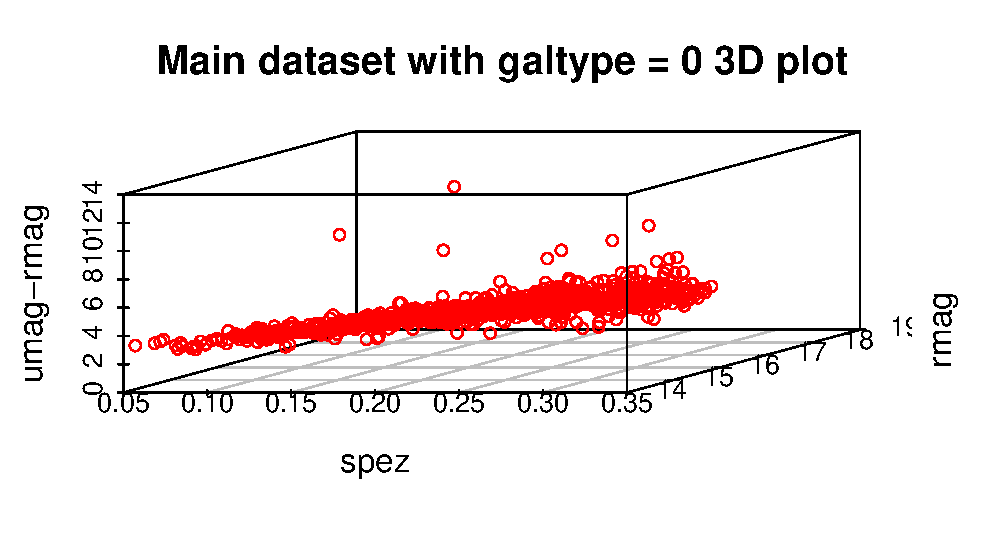
\includegraphics{mainGroup0.pdf}
\caption{ 3D scatter plot for data in \emph{main (galtype= 0)} dataset}

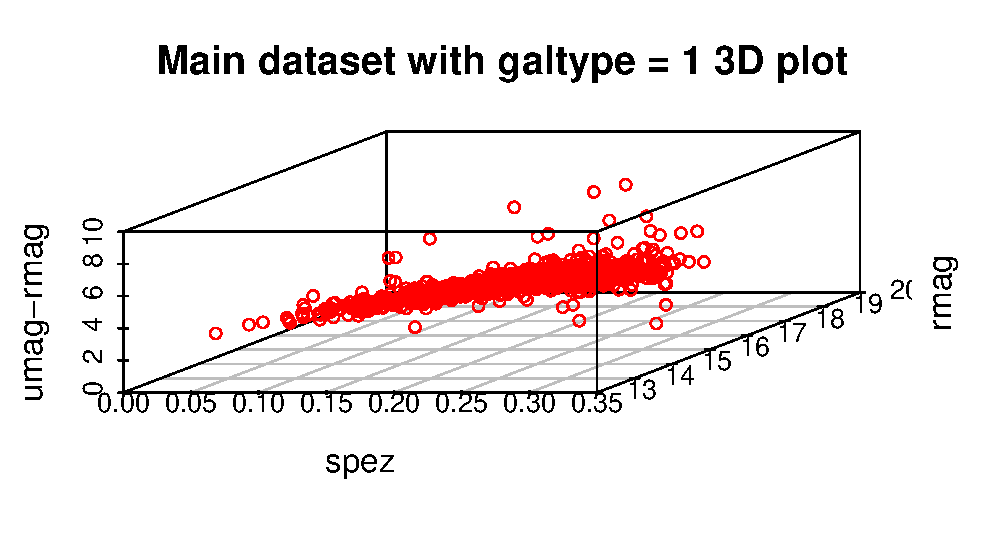
\includegraphics{mainGroup1.pdf}
\caption{ 3D scatter plot for data in \emph{main (galtype= 1)} dataset}

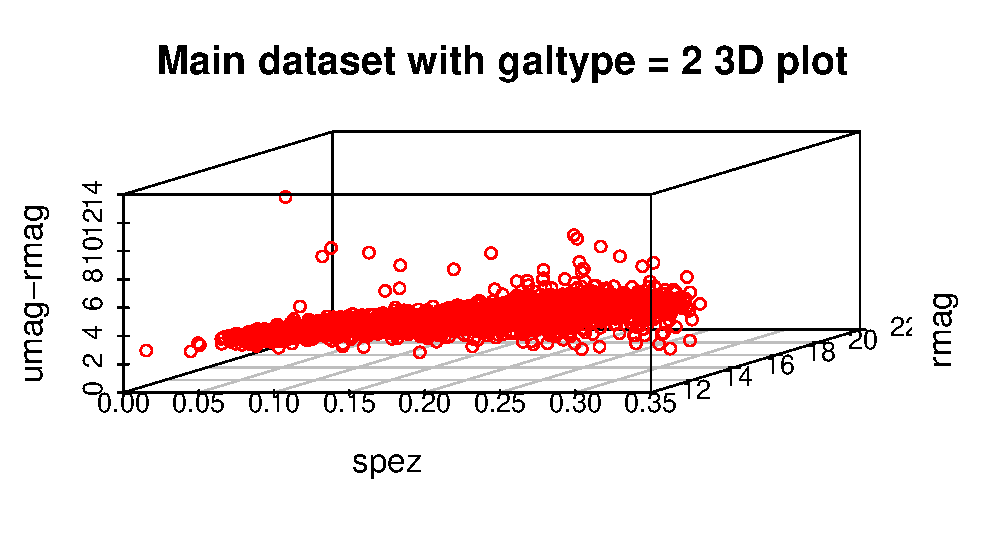
\includegraphics{mainGroup2.pdf}
\caption{ 3D scatter plot for data in \emph{main (galtype= 2)} dataset}
\end{figure}

\pagebreak
	\item Perform data analysis on the features of main and candidate.\\
	\emph{Answer:}
	Below is the correlation between all features in main and in candidate:
\begin{figure}[ht]
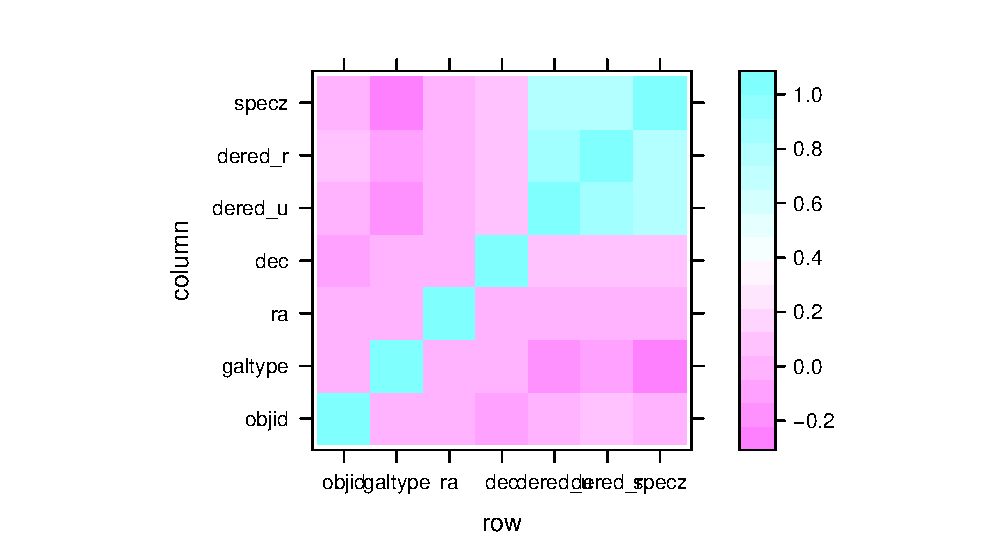
\includegraphics{corMain.pdf}
\caption{ Feature correlation of all Main attributes.}

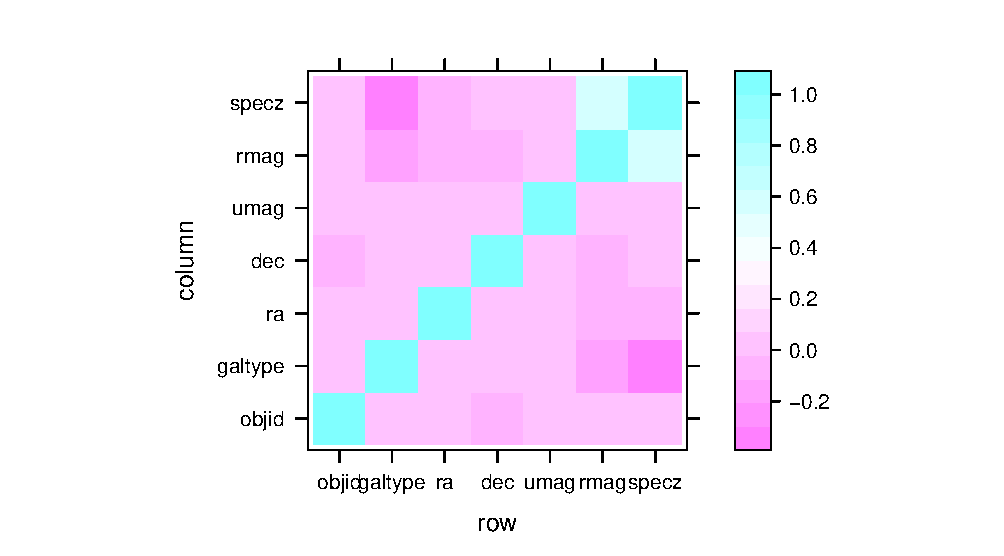
\includegraphics{corCandidate.pdf}
\caption{ Feature correlation of all Candidate attributes.}
\end{figure}

Here cyan refer to positive correlation and pink refers to negative correlation. Moreover, denser the color means higher the correlation. That's why you will se that the diagonal elements are dark cyan. Because they are compared against themselves only. \\

\textbf{My Clustering algorithm bash Shell script} \\
\begin{Sinput}
now=$( date +%d%m%Y-%H%M%S )
outputFile="ClustAlgo_$now.out"
errFile="ClustAlgo_$now.err"

echo "Compiling Code...."
javac -d ./bin ./src/ClusteringAlgo.java

echo "Starting the program in background....."
echo "Execute ps -f the see the status of your code...."
java -cp ./bin ClusteringAlgo > $outputFile 2> $errFile &
\end{Sinput}
\end{enumerate}


\end{document}
